% Appendix A

\chapter{Maps} % Main appendix title

\label{AppendixA} % For referencing this appendix elsewhere, use \ref{AppendixA}

\lhead{Appendix A. \emph{Appendix A}} % This is for the header on each page - perhaps a shortened title

Those three race tracks will be used to evaluate the performance of the controllers. They have been chosen because they present different types of challenges, with combinations of long straight lines and sharp corners.

\section{Formula 1 Track - Red Bull Ring}
The race track for training the controllers is based on the Red Bull Ring race track, located in Austria and hosting the Austrian Grand Prix. the \verb |.png| file that will be used in ROS (Figure \ref{redbull}) is based on \cite{wikiredbull}.

\begin{figure}[H]
\centering
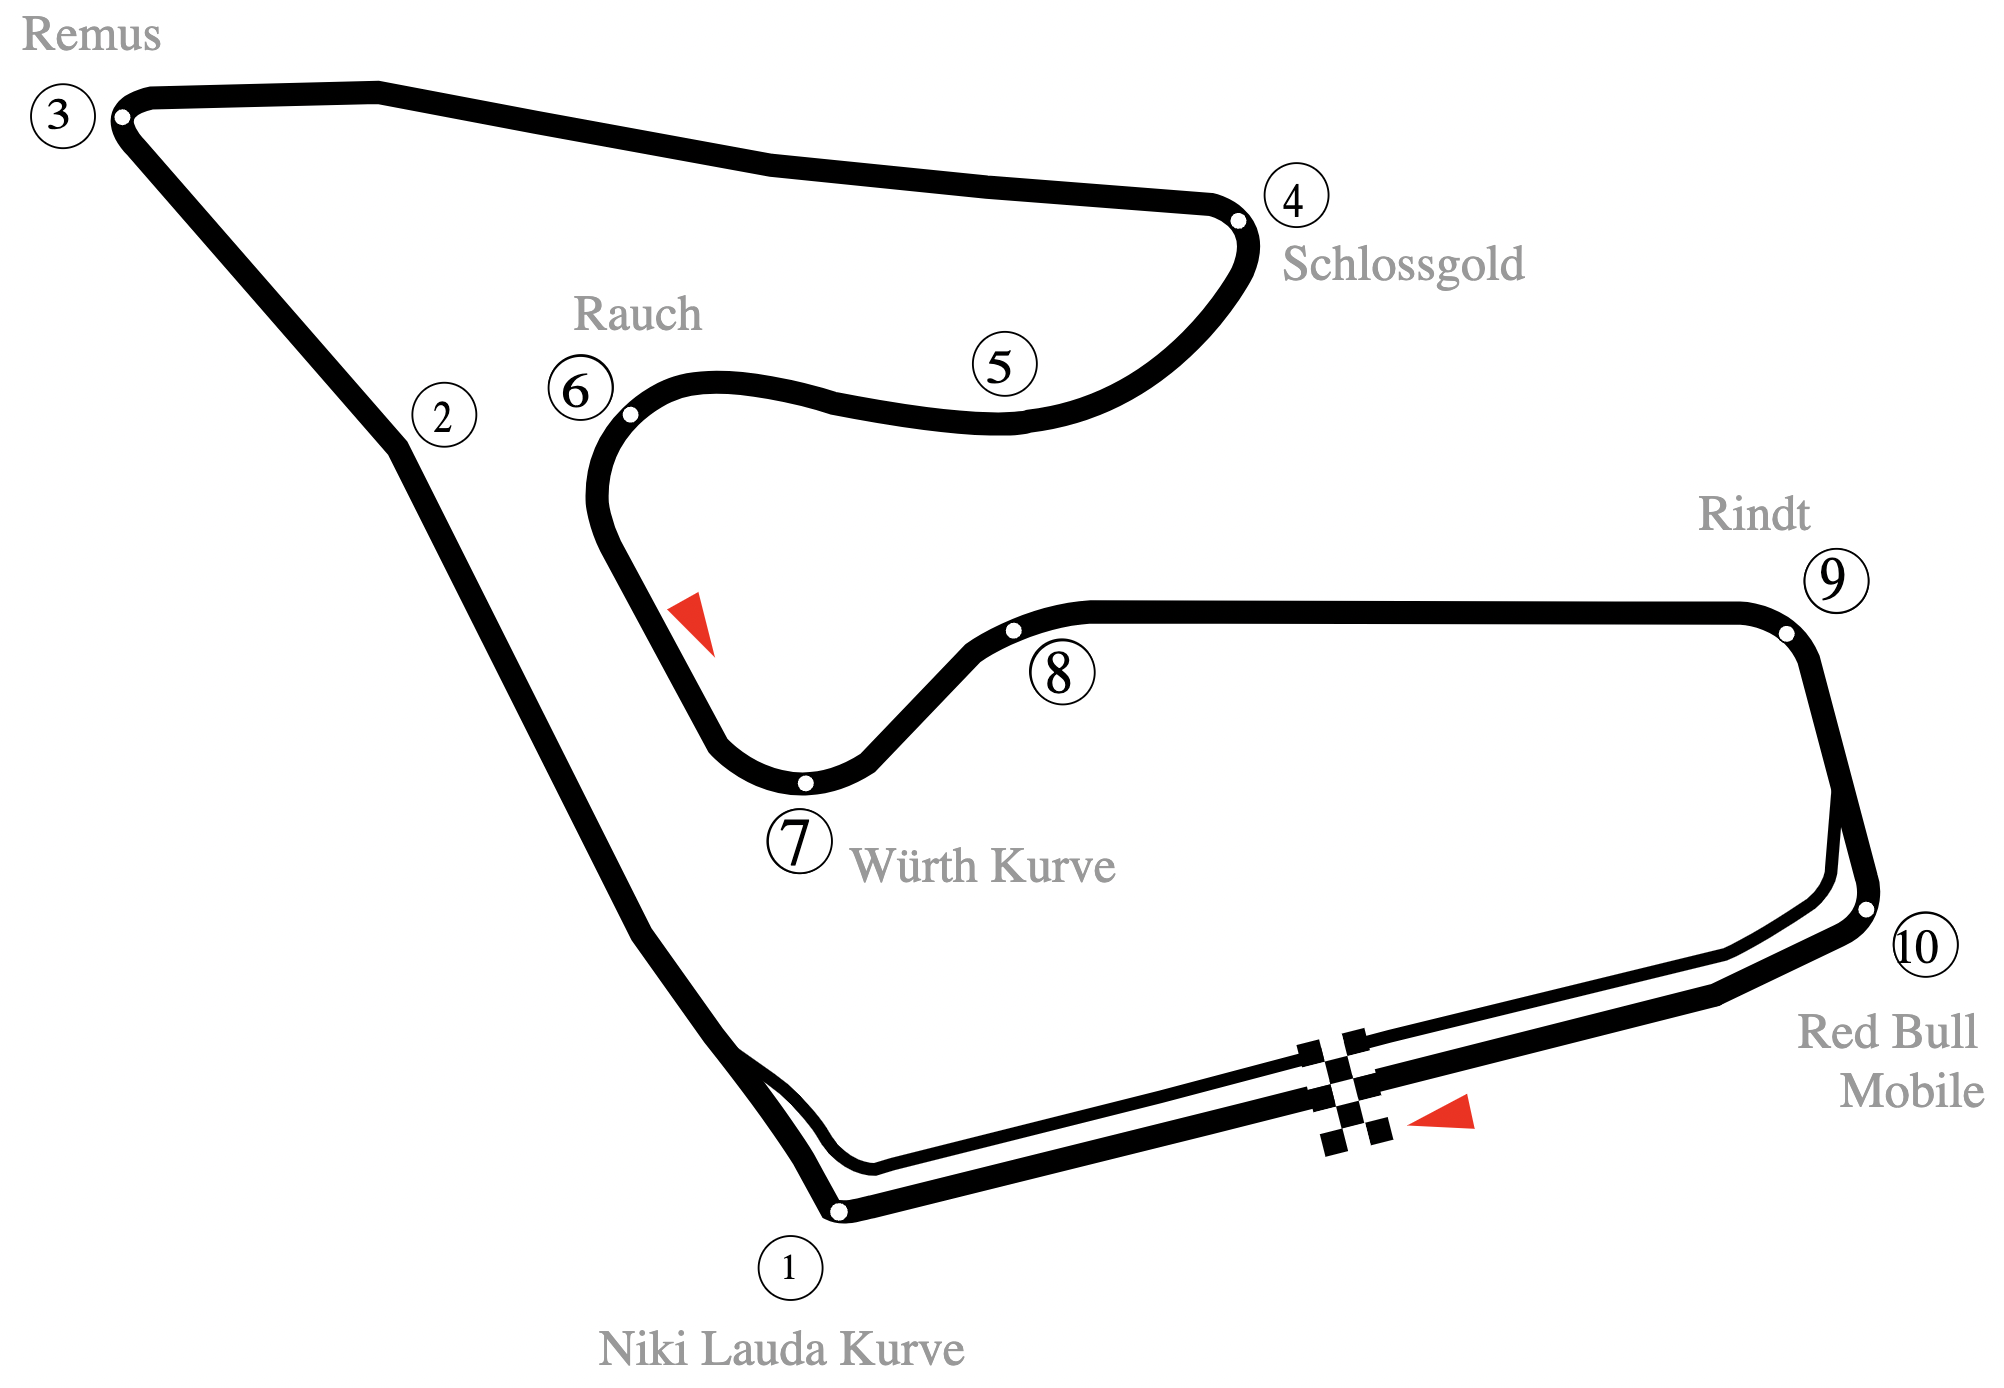
\includegraphics[scale=0.3]{Figures/redbull.png}
\caption{Red Bull Ring Racing Track template from \cite{wikiredbull}}
\label{redbull}
\end{figure}

\section{Formula 1 Track - Silvertone Circuit}
The Silverstone circuit is located in England and hosts the British Grand Prix; the \verb |.png| file that will be used in ROS (Figure \ref{silverstone}) is based on \cite{wikisilver}.

\begin{figure}[H]
\centering
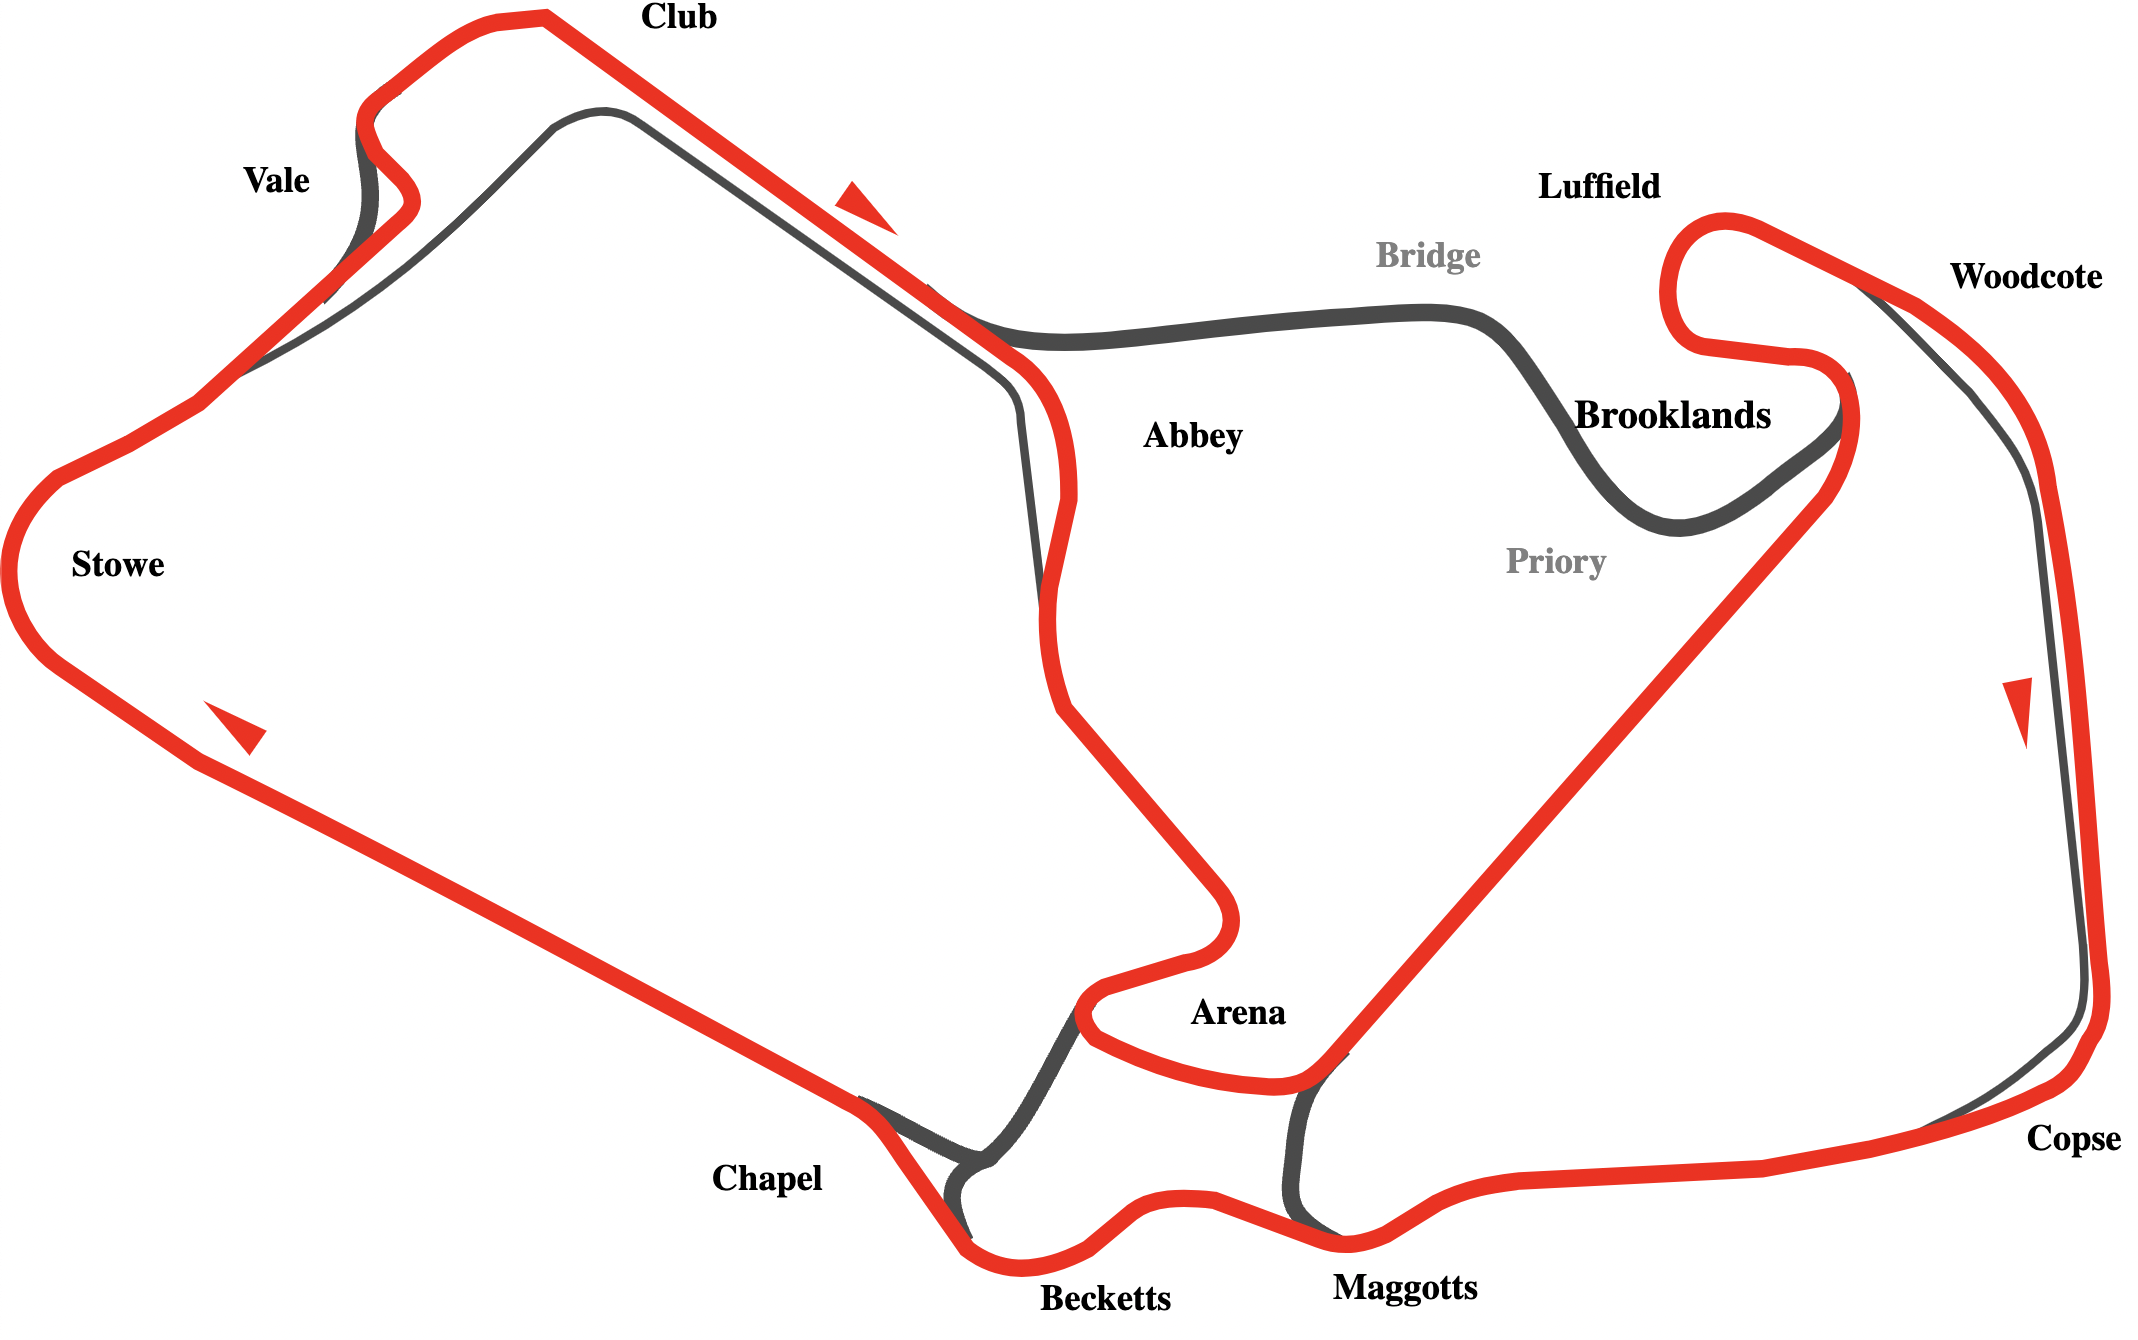
\includegraphics[scale=0.3]{Figures/silverstone.png}
\caption{Silverstone Circuit template from \cite{wikisilver}}
\label{silverstone}
\end{figure}

\section{Formula 1 Track - Circuit de Monaco}
The Circuit de Monaco is located in Monaco and hosts the Monaco Grand Prix; the \verb |.png| file that will be used in ROS (Figure \ref{monaco}) is based on \cite{wikimonaco}.

\begin{figure}[H]
\centering
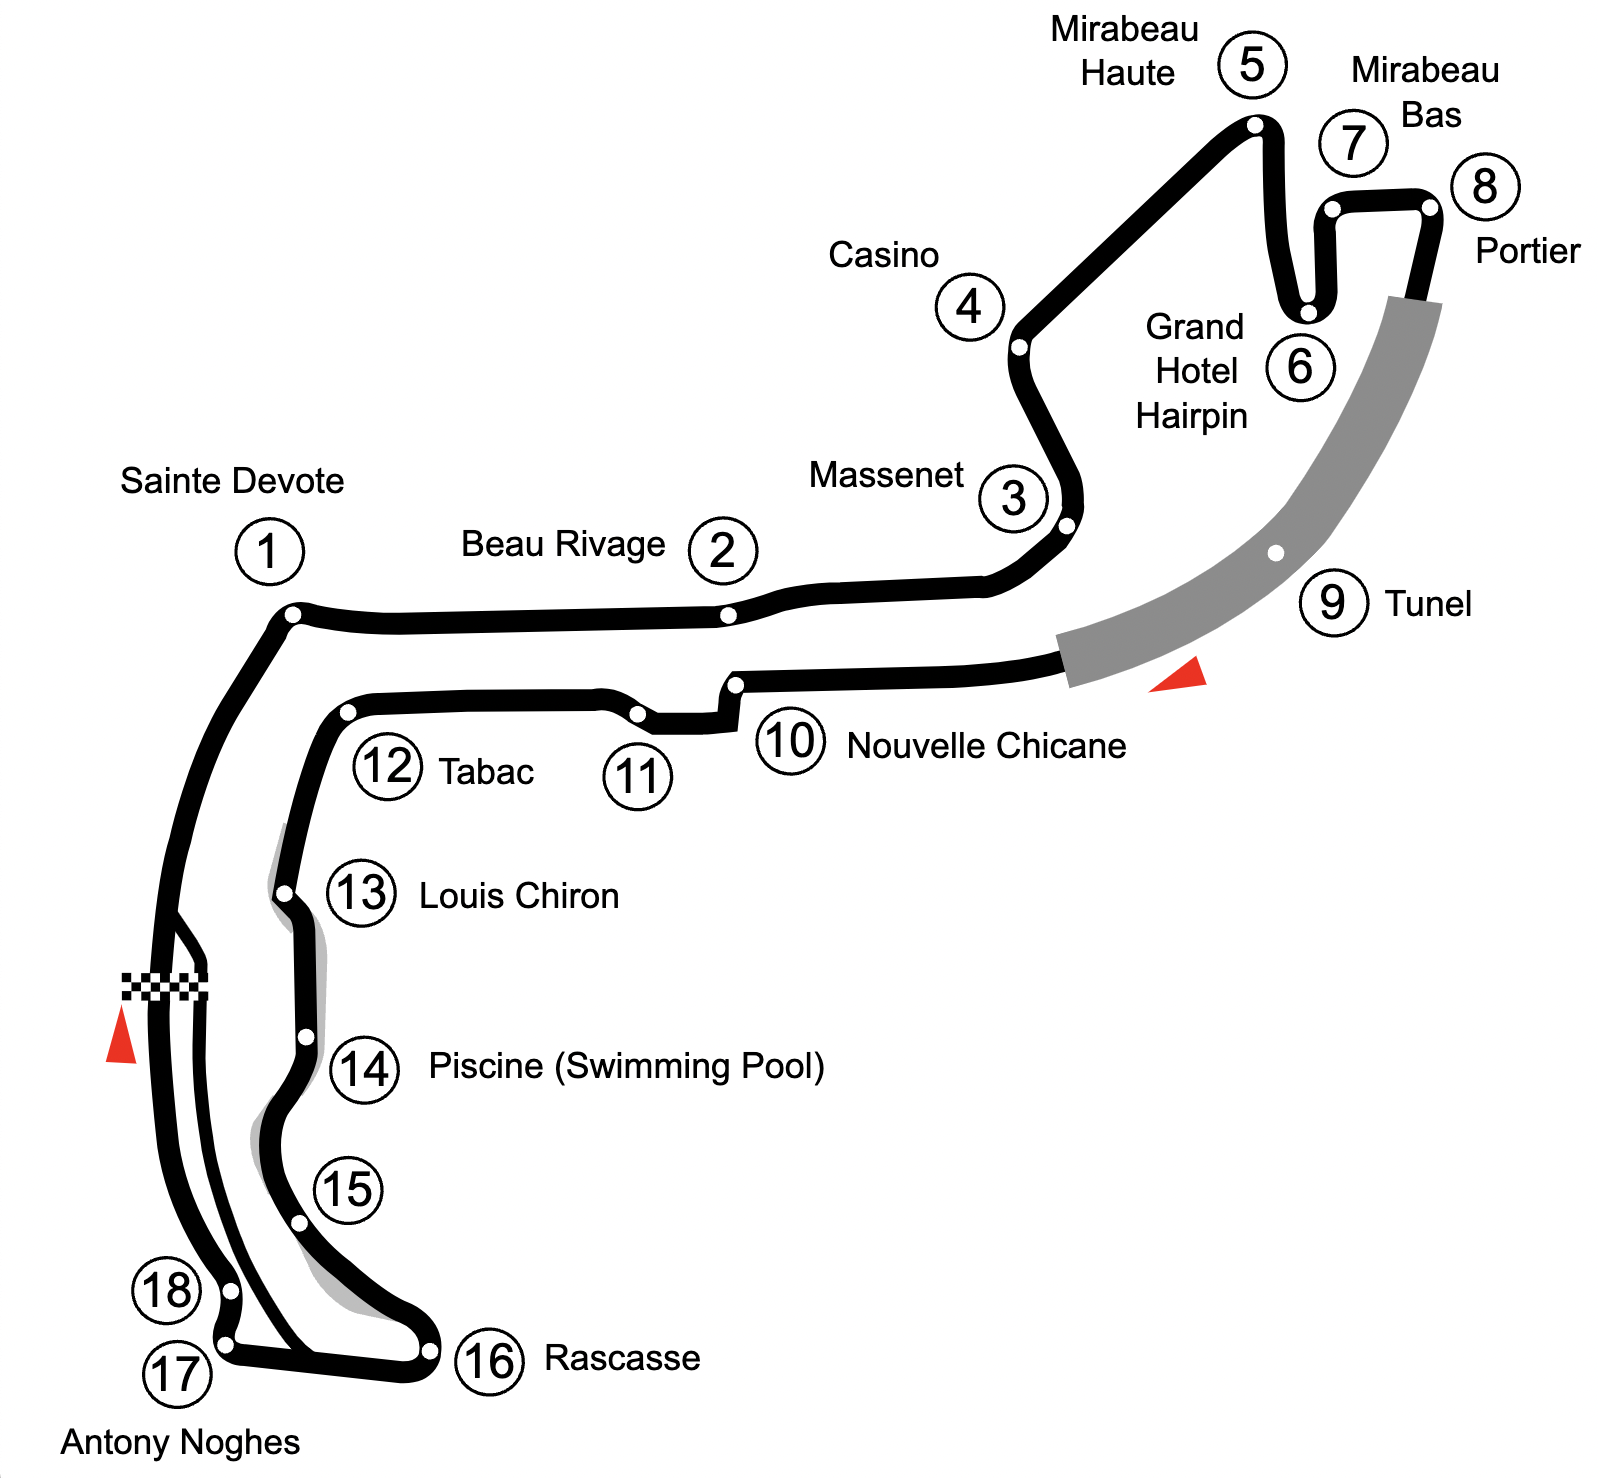
\includegraphics[scale=0.3]{Figures/monaco.png}
\caption{Circuit de Monaco template from \cite{wikimonaco}}
\label{monaco}
\end{figure}

\section{Rectangular Track}
This oval race track was designed by myself, and is used to evaluate the sim-to-real gap.
\begin{figure}[H]
\centering

\includegraphics[scale=0.3]{Figures/round.png}
\caption{Oval-shaped racetrack, inspired by the Mesa Marine Raceway}
\label{oval}
\end{figure}